
%% bare_conf.tex
%% V1.3
%% 2007/01/11
%% by Michael Shell
%% See:
%% http://www.michaelshell.org/
%% for current contact information.
%%
%% This is a skeleton file demonstrating the use of IEEEtran.cls
%% (requires IEEEtran.cls version 1.7 or later) with an IEEE conference paper.
%%
%% Support sites:
%% http://www.michaelshell.org/tex/ieeetran/
%% http://www.ctan.org/tex-archive/macros/latex/contrib/IEEEtran/
%% and
%% http://www.ieee.org/

%%*************************************************************************
%% Legal Notice:
%% This code is offered as-is without any warranty either expressed or
%% implied; without even the implied warranty of MERCHANTABILITY or
%% FITNESS FOR A PARTICULAR PURPOSE! 
%% User assumes all risk.
%% In no event shall IEEE or any contributor to this code be liable for
%% any damages or losses, including, but not limited to, incidental,
%% consequential, or any other damages, resulting from the use or misuse
%% of any information contained here.
%%
%% All comments are the opinions of their respective authors and are not
%% necessarily endorsed by the IEEE.
%%
%% This work is distributed under the LaTeX Project Public License (LPPL)
%% ( http://www.latex-project.org/ ) version 1.3, and may be freely used,
%% distributed and modified. A copy of the LPPL, version 1.3, is included
%% in the base LaTeX documentation of all distributions of LaTeX released
%% 2003/12/01 or later.
%% Retain all contribution notices and credits.
%% ** Modified files should be clearly indicated as such, including  **
%% ** renaming them and changing author support contact information. **
%%
%% File list of work: IEEEtran.cls, IEEEtran_HOWTO.pdf, bare_adv.tex,
%%                    bare_conf.tex, bare_jrnl.tex, bare_jrnl_compsoc.tex
%%*************************************************************************

% *** Authors should verify (and, if needed, correct) their LaTeX system  ***
% *** with the testflow diagnostic prior to trusting their LaTeX platform ***
% *** with production work. IEEE's font choices can trigger bugs that do  ***
% *** not appear when using other class files.                            ***
% The testflow support page is at:
% http://www.michaelshell.org/tex/testflow/



% Note that the a4paper option is mainly intended so that authors in
% countries using A4 can easily print to A4 and see how their papers will
% look in print - the typesetting of the document will not typically be
% affected with changes in paper size (but the bottom and side margins will).
% Use the testflow package mentioned above to verify correct handling of
% both paper sizes by the user's LaTeX system.
%
% Also note that the "draftcls" or "draftclsnofoot", not "draft", option
% should be used if it is desired that the figures are to be displayed in
% draft mode.
%
\documentclass[conference]{IEEEtran}
% Add the compsoc option for Computer Society conferences.
%
% If IEEEtran.cls has not been installed into the LaTeX system files,
% manually specify the path to it like:
% \documentclass[conference]{../sty/IEEEtran}


% Some very useful LaTeX packages include:
% (uncomment the ones you want to load)
\usepackage{graphicx}
\usepackage{amssymb}
\usepackage[noadjust]{cite}
\usepackage{filecontents}
\usepackage[parfill]{parskip}
\usepackage[font=footnotesize]{subcaption}
\usepackage{hyperref}
\usepackage{booktabs}
\renewcommand{\vec}[1]{\mathbf{#1}}

% *** GRAPHICS RELATED PACKAGES ***
%
\ifCLASSINFOpdf
  % \usepackage[pdftex]{graphicx}
  % declare the path(s) where your graphic files are
  % \graphicspath{{../pdf/}{../jpeg/}}
  % and their extensions so you won't have to specify these with
  % every instance of \includegraphics
  % \DeclareGraphicsExtensions{.pdf,.jpeg,.png}
\else
  % or other class option (dvipsone, dvipdf, if not using dvips). graphicx
  % will default to the driver specified in the system graphics.cfg if no
  % driver is specified.
  % \usepackage[dvips]{graphicx}
  % declare the path(s) where your graphic files are
  % \graphicspath{{../eps/}}
  % and their extensions so you won't have to specify these with
  % every instance of \includegraphics
  % \DeclareGraphicsExtensions{.eps}
\fi
% IEEE frowns on bitmapped formats
% which can result in "jaggedy"/blurry rendering of lines and letters as
% well as large increases in file sizes.


% *** MATH PACKAGES ***
%
\usepackage[cmex10]{amsmath}

% *** SPECIALIZED LIST PACKAGES ***
%
%\usepackage{algorithmic}
% algorithmic.sty was written by Peter Williams and Rogerio Brito.
% This package provides an algorithmic environment fo describing algorithms.
% You can use the algorithmic environment in-text or within a figure
% environment to provide for a floating algorithm. 

% *** ALIGNMENT PACKAGES ***
%
\usepackage{array}
% Frank Mittelbach's and David Carlisle's array.sty patches and improves
% the standard LaTeX2e array and tabular environments to provide better
% appearance and additional user controls. 

%\usepackage{mdwmath}
%\usepackage{mdwtab}
% Also highly recommended is Mark Wooding's extremely powerful MDW tools,
% especially mdwmath.sty and mdwtab.sty which are used to format equations
% and tables, respectively.

%\usepackage{eqparbox}
% Also of notable interest is Scott Pakin's eqparbox package for creating
% (automatically sized) equal width boxes - aka "natural width parboxes".
% Available at:
% http://www.ctan.org/tex-archive/macros/latex/contrib/eqparbox/


%\usepackage[tight,footnotesize]{subfigure}

%\usepackage[caption=false, font=footnotesize]{subfig}
% subfig.sty, also written by Steven Douglas Cochran, is the modern
% replacement for subfigure.sty. However, subfig.sty requires and
% automatically loads Axel Sommerfeldt's caption.sty which will override
% IEEEtran.cls handling of captions and this will result in nonIEEE style
% figure/table captions. To prevent this problem, be sure and preload
% caption.sty with its "caption=false" package option. This is will preserve
% IEEEtran.cls handing of captions. Version 1.3 (2005/06/28) and later 
% (recommended due to many improvements over 1.2) of subfig.sty supports
% the caption=false option directly:
%\usepackage[caption=false,font=footnotesize]{subfig}

\usepackage{fixltx2e}

%\usepackage{stfloats}
% stfloats.sty was written by Sigitas Tolusis. This package gives LaTeX2e
% the ability to do double column floats at the bottom of the page as well
% as the top. (e.g., "\begin{figure*}[!b]" is not normally possible in
% LaTeX2e). It also provides a command:
%\fnbelowfloat

\usepackage{url}

% correct bad hyphenation here
\hyphenation{op-tical net-works semi-conduc-tor}

\begin{document}
%
% paper title
% can use linebreaks \\ within to get better formatting as desired
\title{Energy Forecasting for the Global Energy Forecasting Competition 2014\\[10pt]\Large{\emph{Semester Project Report}}}

% author names and affiliations
% use a multiple column layout for up to three different
% affiliations
\author{\IEEEauthorblockN{Fabian Brix\\MSc Candidate}
\IEEEauthorblockA{School of Computer \& Communication Sciences\\
Swiss Federal Institute of Technology Lausanne\\
fabian.brix@epfl.ch}
%\and
%\IEEEauthorblockN{Homer Simpson}
%\IEEEauthorblockA{Twentieth Century Fox\\
%Springfield, USA\\
%Email: homer@thesimpsons.com}
}

\maketitle

\begin{abstract}
%\boldmath
The abstract goes here.
\end{abstract}
% IEEEtran.cls defaults to using nonbold math in the Abstract.
% This preserves the distinction between vectors and scalars. However,
% if the conference you are submitting to favors bold math in the abstract,
% then you can use LaTeX's standard command \boldmath at the very start
% of the abstract to achieve this. Many IEEE journals/conferences frown on
% math in the abstract anyway.

% no keywords

% For peer review papers, you can put extra information on the cover
% page as needed:
% \ifCLASSOPTIONpeerreview
% \begin{center} \bfseries EDICS Category: 3-BBND \end{center}
% \fi
%
% For peerreview papers, this IEEEtran command inserts a page break and
% creates the second title. It will be ignored for other modes.
\IEEEpeerreviewmaketitle

\section{Introduction}
\subsection{GEFCom 2014}
The Global Energy Forecasting Competition (GEFCom 2014) is the second edition of a competition first held on Kaggle in 2012 that attracted hundreds of participants contributing many novel ideas to the energy forecasting field. The second edition lasted from 08/15/2014 to 12/15/2014 and was sponsored by several IEEE bodies and the International Journal of Forecasting. It included four competition tracks: electric load, electricity price, wind power and solar power forecasting. The respective data was published on the community platform of crowdanalytix.com on a weekly basis during the competition. The format of the competition was that of rolling forecasting requiring contestants to submit the next period of interest to forecast a day before the next set of data was published. To appear on the final leaderboard the contestants had to submit 99 quantiles for each step throughout the forecast horizon. In the course of this semester project we focused solely on the electric load forecasting track. This track had a weekly forecast horizon of one month and consisted of three trial periods and twelve competitive periods. In order to feature on the final leaderboard nine competitive submissions were required. Due to our lack of familiarity with the subject, participating in the competition was not prioritized after initial attempts. Instead the focus was on comparison of the performance of different methods on the whole dataset via cross validation.
%The topic of the probabilistic electric load forecasting track is to forecast the probabilistic distribution (in quantiles) of the hourly loads for one utility on a rolling basis
%Historical Data Release (Competition Starts) 8/15/2014
%Evaluation Period Starts 9/14/2014
%Registration Deadline 10/10/2014
%Evaluation Period Ends 12/6/2014
%Final Report and Code Due (Competition Ends) 12/15/2015

\subsection{Short Introduction to Energy Load Forecasting}
Before we review related work we are going to introduce the area of Energy Load Forecasting. Load forecasting, as it is commonly referred to, is usually concerned with the prediction of hourly, daily, weekly, and annual values of the system demand and peak demand of an electric utility \cite{Fan2010}. Such forecasts are sometimes categorized as short-term (up to 1 week), medium-term (1 week - 1 year) and long-term (> 1 year ) forecasts, depending on the time horizon. In the load forecasting track of GEFCom 2014 we are concerned with forecasting the daily electricity load of a utility for a whole month on a rolling basis given the data of the previous years. The task is therefore on the threshold between short-term and medium-term load forecasting.\par
Load Forecasting is necessary for the planning of energy system and their effective operation and maintenance. Forecasting accuracy therefore has a major impact on electric utilities and their regulators. In case of overestimation of future energy load, utility providers will operate too many units possibly driving energy demand and in case of long-term forecasts investment in the construction of new infrastructure can be wasted. Underestimation leads ot unmet demand and systems that are vulnerable to crashes.  
The output of such forecasts can either be point forecasts or estimates of the probability distribution of values of future demand or load as required during GEFCom 2014.
Electricity load follows a nonlinear, volatile pattern subject to several exogenous variables such weather conditions, randomness in human behavior leading to randomness in demand and economic conditions and demographic changes. In GEFCom 2014 the exogenous variables are limited to weather conditions in the form of recorded temperature at several sites and calendar effects such as the effects of weekends and holidays on the electricity demand.
In this report we analyse the predictions produced by algorithms that are capable of capturing the nonlinear dependencies between these exogeneous variables and the load such as General Additive Models, Random Forests, Multilayer Perceptrons. We do not strive to build any algorithms ourselves, but employ the various implementations in R of the mentioned algorithms.

LOAD vs DEMAND?? == consumption vs. demand??

%Objective
%The topic of the probabilistic electric load forecasting track is to forecast the probabilistic distribution (in quantiles) of the hourly loads for one utility on a rolling basis.

\section{Review of Related Work}
Get relevant sections from Tao Hong's working paper literature review
Day of the Week etc.
Hyndman for more features
Review previous work from Gefcom 2012 and beyond including papers with related approaches including but not necessarily limited to those that can be found under the following link: http://blog.drhongtao.com/2014/08/recommended-papers-for-gefcom2014-contestants.html. Distinguish between approaches to temperature and load prediction.\par
Probabilistic Electric Load Forecasting: A Tutorial Review
%https://onedrive.live.com/view.aspx?resid=BCA4C2DC57A4CB2A!519&app=WordPdf
contains literature review for longterm probabilistic load forecasting

Tao Hang, Jason Wilson:
Long Term Probabilistic Load Forecasting and Normalization With Hourly Information
but papers is on Long Term Electric Load Forecasting: 1-X years \cite{Hong2014Normalization}

Rob Hyndman, Shu Fan
Density Forecasting for Longterm Electricity Demand
Source for calendar effects \cite{Hyndman2010}

Shu Fan, Rob Hyndman
Short-term load forecasting based on a semi-parametric additive model \cite{Fan2010}

\section{Dataset and Evaluation Metrics}
\subsection{Dataset}
%Forecast horizon: 1 month
The dataset provided by GEFCom 2014 includes hourly historical load and weather data of a utility in an undisclosed area on the east coast of the United States of America. The 25 weather stations in the dataset provide historical temperature for their respective zones. However, the load data consists only of the system level load in Mega Watts (MW) and not all of the zonal level load series. Therefore, forecasts in the context of Smart Grid Technology are not required. The temperature data made available consists of 25 series of temperature data in Fahrenheit from the 25 different weather statios dating from 01/01/2001 to 12/01/2011. The load data of the utility is recorded starting from the 01/01/2005 at 1am.\par
The complete data set acted both as training and validation set except for the first and last month of the data published for the reason that the data was released on a weekly basis. It consists of 15 spreadhseets in the format of Comma-Seperated Values (CSV) for the load forecasting track. The first spreadsheet contains data starting from 01/01/2001 up until midnight on the 10/01/2014 at 1am from when on the incremental spreadsheets released every week contain only one month of data.\par
The forecasts were required to be made starting from 10/01/2010 on a monthly rolling basis for 15 months. The nature of the data provided required the contestants to produce their own temperature forecasts for the month ahead in the dataset.\par

LOAD: one utility! Domestic + Industrial --> less nice patterns? --> less impact of holiday effect?

%

\subsection{Evaluation Metrics}
The comptetition requries each the participants to provide percentile forecasts, that is forecasts of the quantiles $\tau=0.01, 0.02, \dots, 0.99$ with natural lower and upper bounds.
The Evaluation Metric employed to score the contestants' submissionsis the tilted loss/error function also known as the pinball loss/error function. In the following paragraphs let $y$ denote an observation and $\hat{y}$ denote a corresponding forecast while $\xi$ is defined as the residual $y-\hat{y}$.\par
%For a quantile forecast q_a with a/100 as the target quantile, this score L is defined as:
%L(q_a, y) = (1 - a/100) * (q_a - y), if y<q_a;
                %a/100 * (y - q_a), if y>=q_a
%where y is the observation used for verification, a = 1, 2, ..., 99.
\[
  L_{\tau}(\xi)=\begin{cases} \tau \xi & \text{if } \xi \geq 0 \\
                                          (\tau-1)\xi & \text{if } \xi < 0 
                                  \end{cases} \quad\text{where } \xi=(y-\hat{y})
\]
%\tau ist Steigung wenn \xi>=0 und Gefälle wenn \xi<0
To evaluate the full predictive densities, this score is then averaged over all target quantiles, from 0.01 to 0.99, for all time periods throughout the forecast horizon. The lower the pinball score, the better the forecast.

\begin{figure}[ht!]
\centering
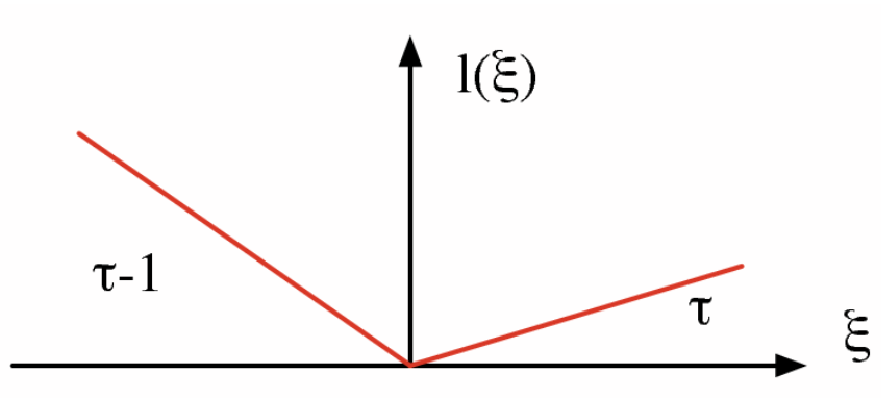
\includegraphics[width=\linewidth]{gfx/pinball.pdf}
\caption{The tilted loss function for 50th, $\tau=0.5$, and 75th, $\tau=0.75$, quantile \cite{Takeuchi2005}.}
\label{fig:pinball}
\end{figure}
%TODO: Include the proof for why the ``pinball'' loss estimates the $\tau$-quantile \cite{Takeuchi2005}.\par
\paragraph{Why Quantile Forecasting?}
\textit{In today's competitive and dynamic environment, more and more decision making processes in the power and energy industry are relying on probabilistic forecasts. The applications of probabilistic energy forecasts spread across planning and operations of the entire energy value chain.}

In our own evaluation of forecasts, we further use some well-established point error metrics, for the simple reason that we generate our quantile predictions starting from a point prediction. The measures are the Mean Average Error (MAE), Root Mean Squared Error (RMSE) and Mean Absolute Percentage Error (MAPE).\par
The MAE and RMSE measures are the two most common scale-dependent errors, meaning that the residuals $\xi_i$ (for ith observations) are on the same scale as the data. Hence, MAE and RMSE are in units of Fahrenheit or Mega Watt for our data set. 
\[
  \text{MAE}=\mathbb{E}[\xi_i]
\]
\[
  \text{RMSE}=\sqrt{\mathbb{E}[\xi_i]}
\]
As a percentage error the MAPE measure is scale-independent. In our case it is useful for giving an immediate sense of the relative magnitude? of the error.
\[
  \text{MAPE}=\mathbb{E}\left[\left| \frac{100\xi_i}{y_i} \right|\right]
\]
The measure is undefined for $y_i=0$. Fortunately, in our dataset all values are several integers larger than zero for both load and temperature series so that the measure is neither undefined or affected by extreme values.
%source: Rob Hyndman, Forecasting principles and practice, https://www.otexts.org/fpp/2/5

\subsection{Data Cleaning}
An annoying feature of the dataset is that the timestamps are not saved in the international ISO 8601 standard, but as ``MMddYYYY H:m'' without leading zeros for both days and months. Fortunately, the dataset was provided continuously without gaps and therefore the problem could be easily solved by hard-coding the first and last datetimes and using these to generate the needed sequence of datetimes.n
%found a way to automatically solve the problem through the linkedin group and a question a participant asked on stackoverflow (http://stackoverflow.com/questions/25386730/parsing-ambiguous-timestamps). 
%However, had to make slight modifications to make it work
%Still didn't work 100%, lost one week on this

\subsection{Temperature Data Selection}
%$Corr_X(m) = \frac{\mathbb{E}\[X_t-\mu_x)(X_{t+m})\]}{\var_X}$
We use the average temperature of all weather stations at any hour $i$ as the basis series for our temperature forecasts (Figure \ref{subfig:avg-temp-2012}).
As the basis for the load forecasting we use the average over all the temperature stations provided in the dataset. In other words, we use the average district temperature to predict the district utility load.\par

\cite{Fan2010} temperature highly correlated $\rightarrow$ use average
however, did not use temperature differences: would have led to 25x25 more features

In another approach we compute the cross-correlations of the 25 weather station's series (Figure \ref{fig:temp-stations-cc}). These suggest that the district temperature can be explained on average to over 90\% by the first series.\par
\begin{figure}[ht!]
\centering
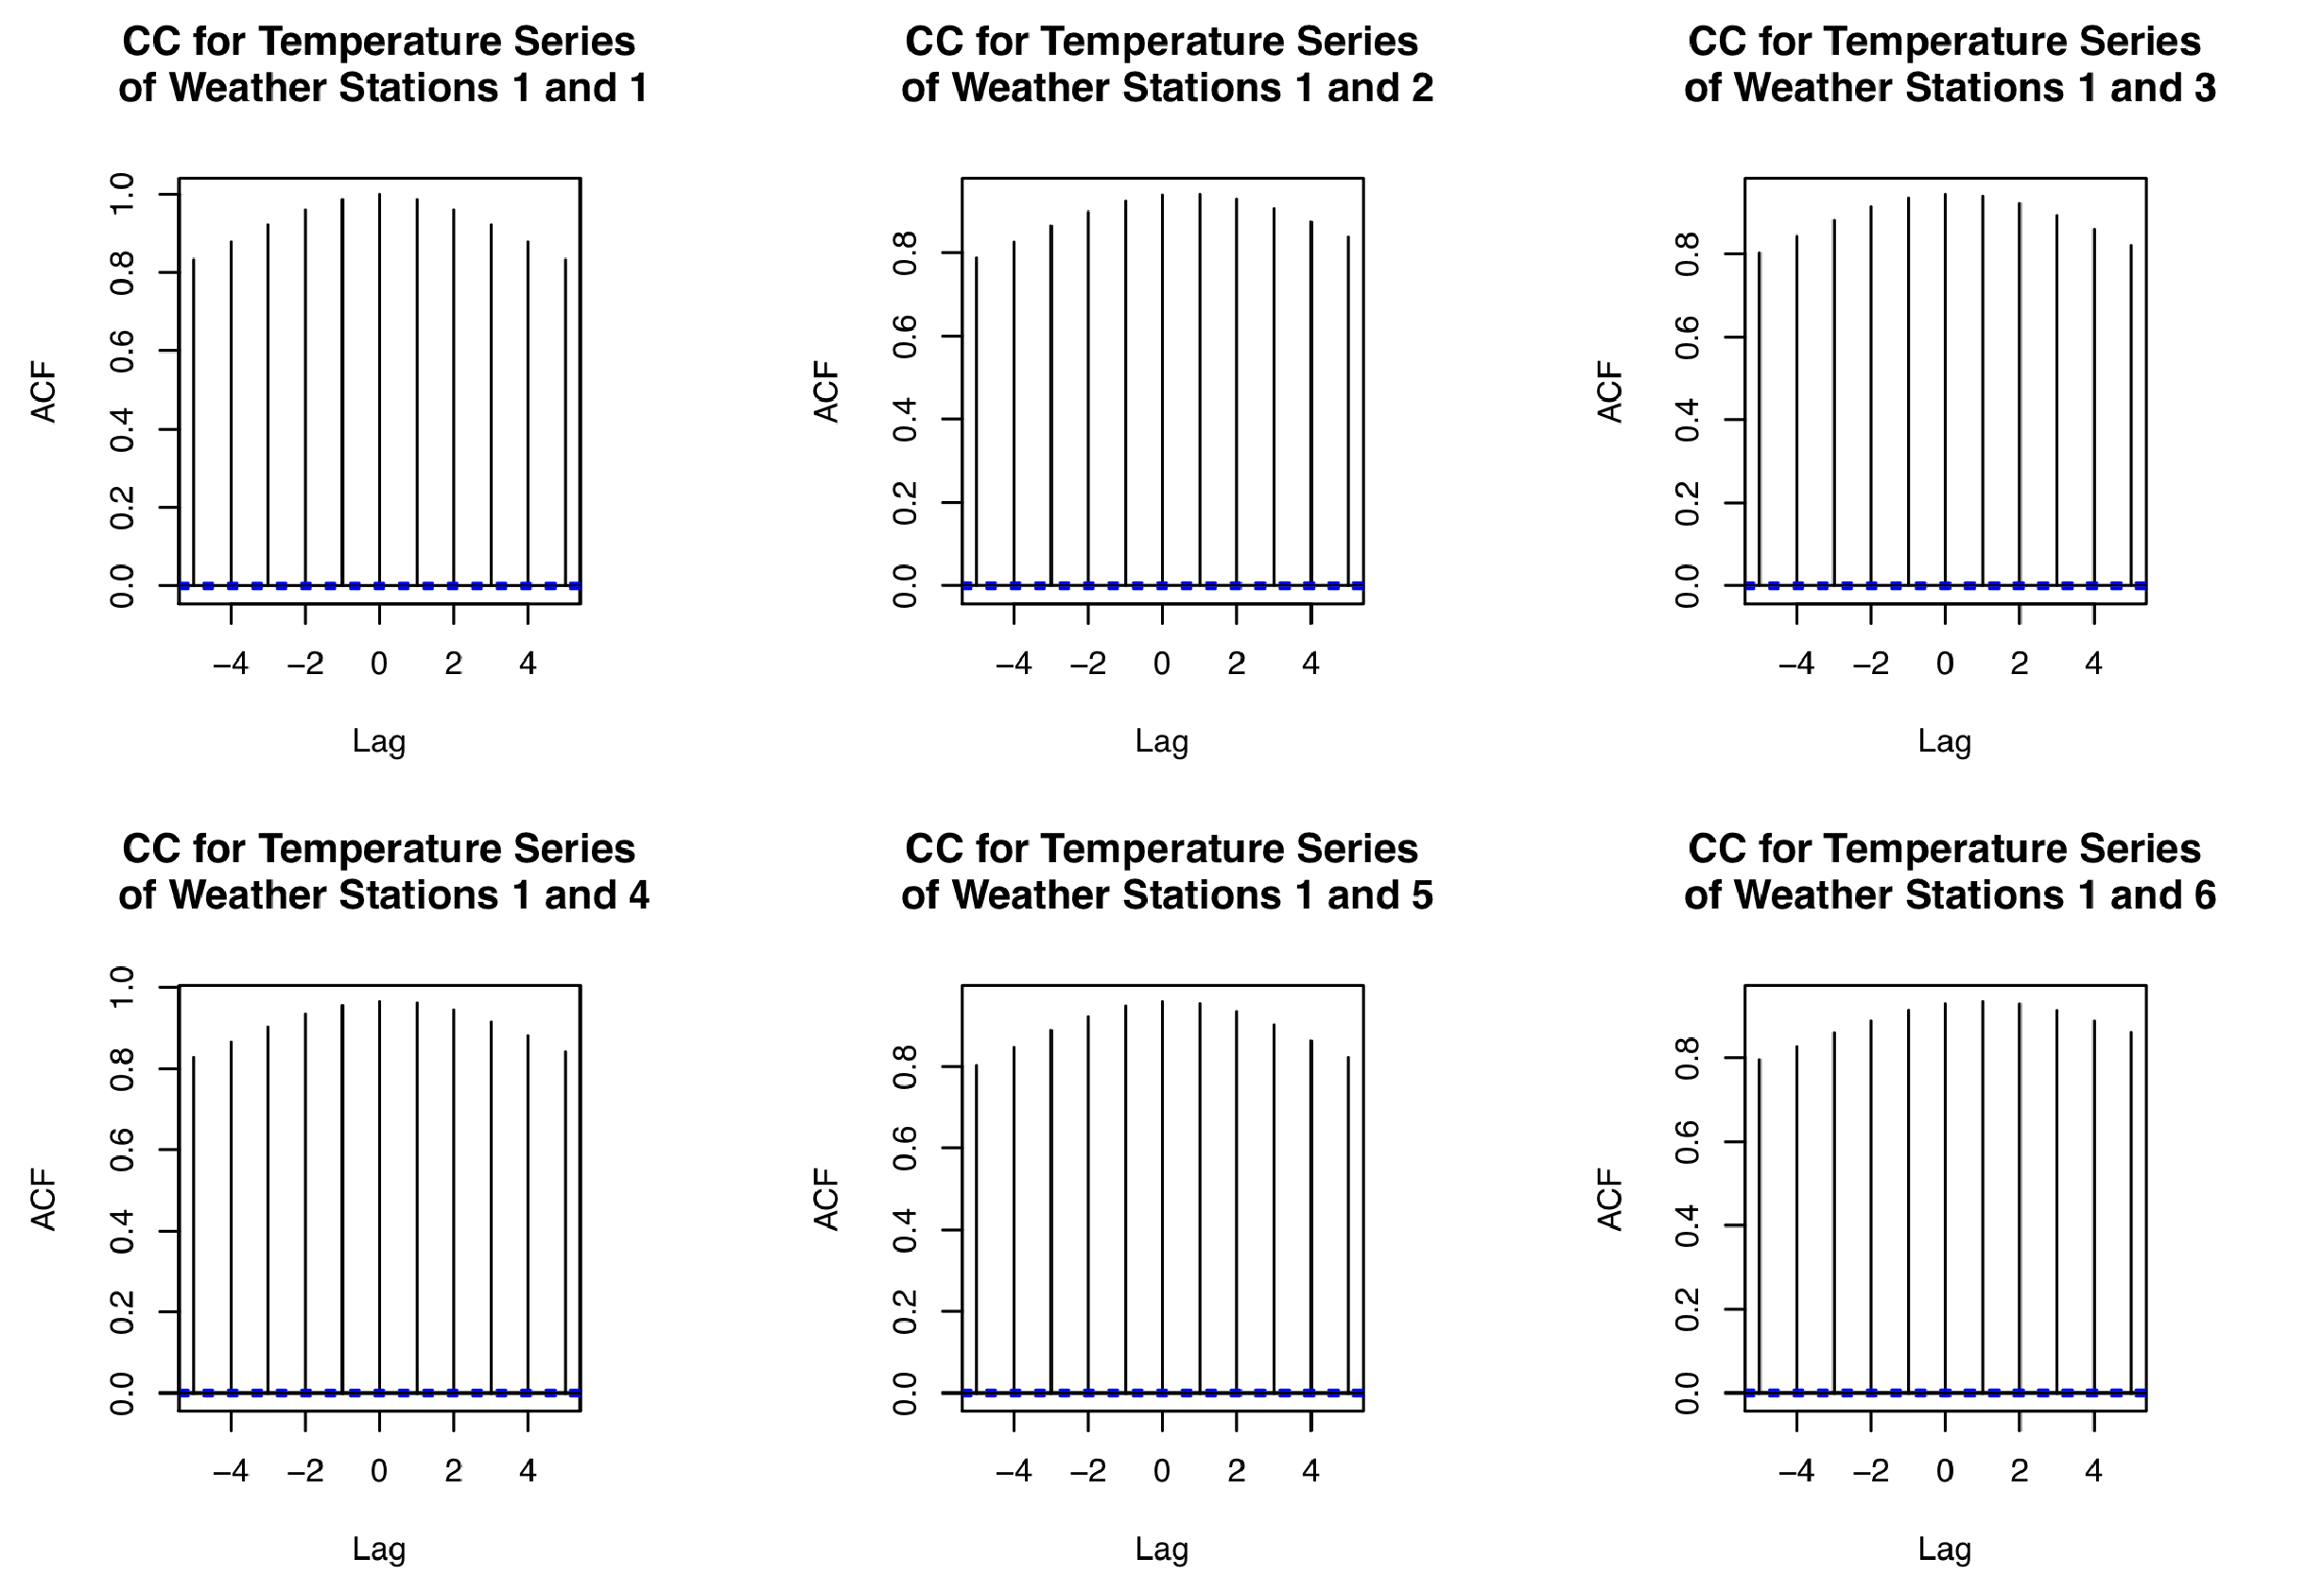
\includegraphics[width=\linewidth]{gfx/weather-station-cc-plots_series1-6_lag5.pdf}
\caption{Cross Correlation Plots of Temperature Station 1 Series with Series of Temperature Stations 1-6. Cross Correlations for Stations 7-25 ommitted for convenience of display.}
\label{fig:temp-stations-cc}
\end{figure}
A temperature of 60 degrees Fahrenheit would therefore allow for an error of maximum 6 degrees of Fahrenheit or 3 degrees Celsius respectively. As we will see later in this report this error is negligible when taking into account the inaccuracy of/the error introduced in the temperature prediction.\par

\begin{figure}[!ht]
\centering
\begin{subfigure}[b]{.6\linewidth}
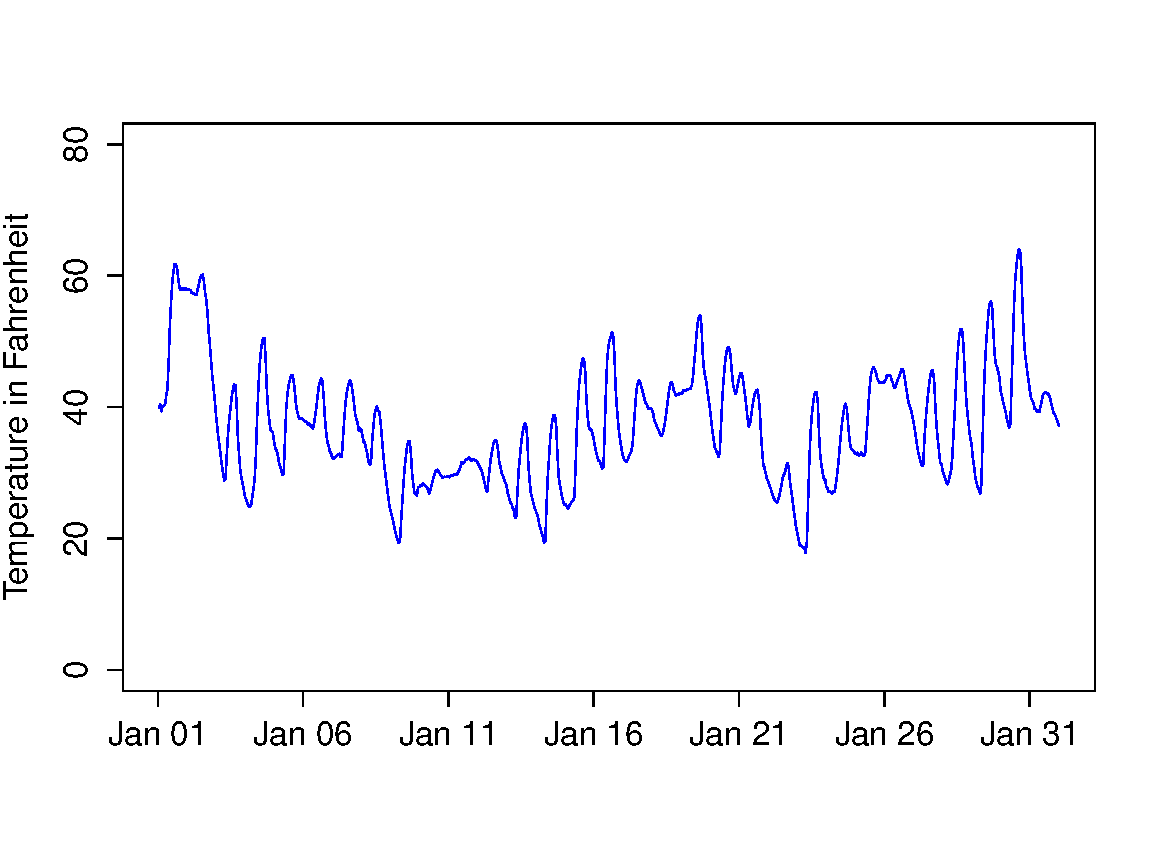
\includegraphics[width=\linewidth]{gfx/avg-temp-2011.pdf}
\caption{Average Zonal Temperature during July 2011}
\label{subfig:avg-temp-2012}
\end{subfigure}
\quad
\begin{subfigure}[b]{.6\linewidth}
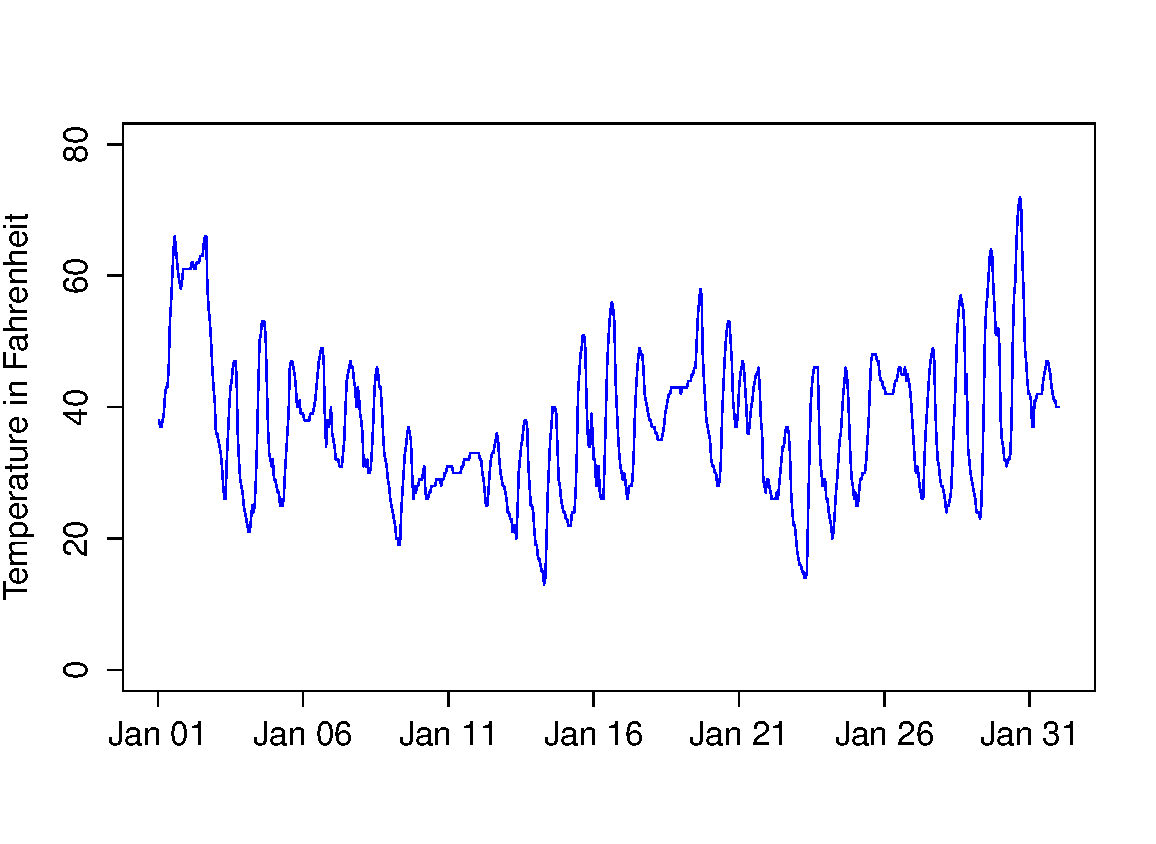
\includegraphics[width=\linewidth]{gfx/temp-station1-2011.pdf}
\caption{Temperature of 1st Weather Station during July 2011}
\label{subfig:temp-station1-2012}
\end{subfigure}
\end{figure}

\section{Feature Selection}
In the following paragraphs we explain the methodology we use to obtain our final feature selection for both temperature and load forecasting. The choice of features is limited to calendar features for temperature forecasting, because the only additional data allowed in the competition are Federal US holidays and the forecasting horizon is set to 1 month ahead.
\subsection{Time Lags}
First of all, we want to find out which previous values can be useful in a prediction. Given a time horizon of 1 month we would like to forecast the whole month using only one model for reasons of convenience. This circumstance induces a time lag of minimum 28 days for the month of february. For simplicity of implementation we define the same minimum lag of 31 for every month of the year.   
In order to choose the lag variables we interprete the cross-correlation of observations $y_i$ and $y_{i-k}$, for different hourly lags $k=1,2,..$, of both temperature and load time series in (Figure \ref{fig:temp-lags}).
This cross-correlation of observations is known in statistics as Autocorrelation and demonstrates the similarity of observations in a series as a function of the time lag between them.
% series are not Second Order Stationary Processes?
%When your data is nonstationary (inhomogeneous), autocorrelation can still be defined and computed, but will now depend on the pivot (=reference) point as well, nut just the distance (=delay, lag) between points. As a result, the autocorrelation becomes a functional, no longer a function. In the discretized (sampled) case, this functional becomes a matrix.
Using the empirical mean and standard deviation of our target series $Y=\{y_1, y_2, \dots, y_i, \dots, y_N\}$ we can compute the autocorrelation for lag k with:
\[
  \mathcal{R}(k)=\frac{\mathbb{E}\left[(y_i-\mu)(y_{i-k}-\mu)\right]}{\sigma^2}
\]

As can be seen in both figure \ref{subfig:avg-temp-7days} and \ref{subfig:temp-station1-7days} the highest autocorrelations occur with a frequency/periodicity of 24 hours. Therfore we choose 24 hours as the basis constant for selecting the time lags of our predictions. The average temperature series in the former figure displays less variance in the correlations than the latter because the hourly temperature is less extreme due to zonal averaging. 

\begin{figure}[!ht]
\centering
\begin{subfigure}[b]{.49\linewidth}
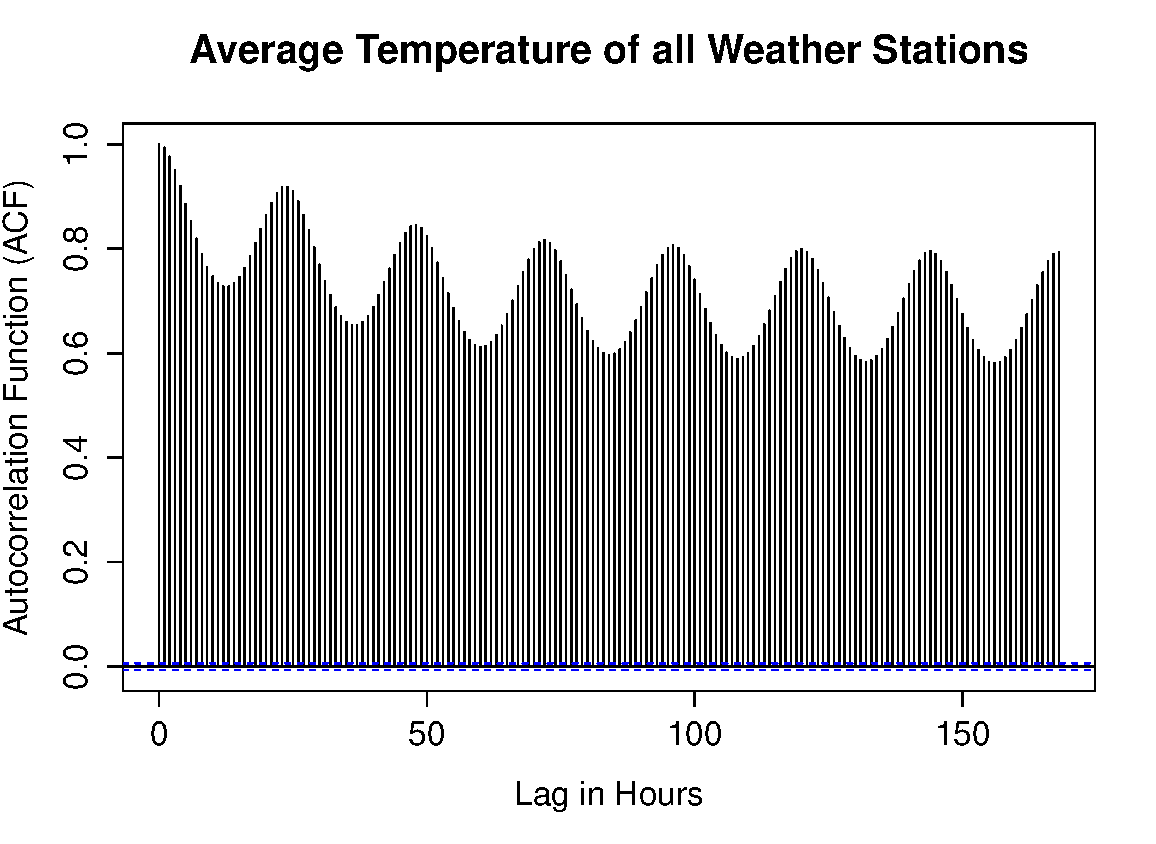
\includegraphics[width=\linewidth]{gfx/acf_avg_temp_7days.pdf}
\caption{7 days Autocorrelation}
\label{subfig:avg-temp-7days}
\end{subfigure}
\begin{subfigure}[b]{.49\linewidth}
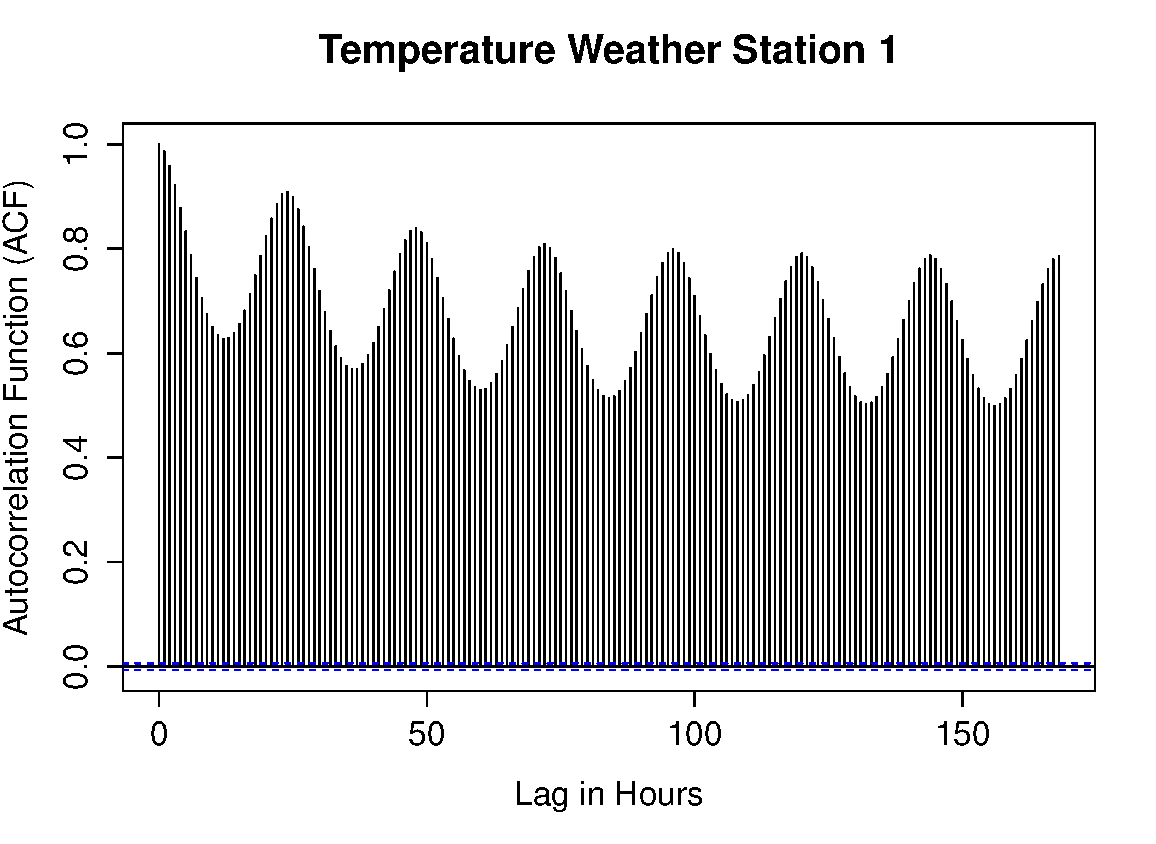
\includegraphics[width=\linewidth]{gfx/acf_temp_station1_7days.pdf}
\caption{7 days Autocorrelation}
\label{subfig:temp-station1-7days}
\end{subfigure}
\caption{..}
\label{fig:temp-lags}
\end{figure}

Figure \ref{fig:acf-load} shows the autocorrelation function of the load series for different maximum lags. As can be seen the load correlations also have a periodicity of 24 hours (\ref{subfig:acf-load-7days} ). The other subfigures show that after an initial exponential decrease the correlations decrease near linearly. Since the type of day has an influence on the utility load (Section \ref{sec:calendar}), we set the basis for time lags to $7\cdot24$ hours for the load and the minimum time lag for monthly load forecasts therefore to 35 days.

\begin{figure}[!ht]
\centering
\begin{subfigure}[b]{.49\linewidth}
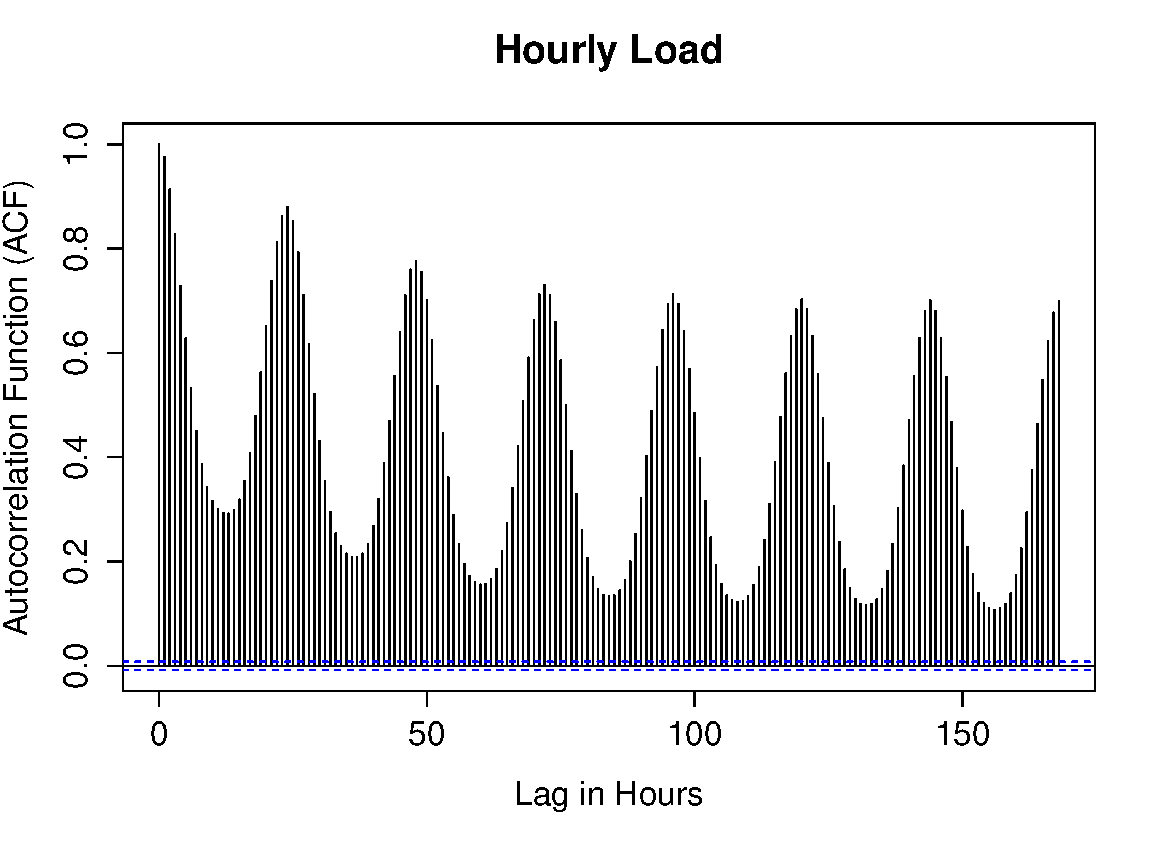
\includegraphics[width=\linewidth]{gfx/acf-load-7days.pdf}
\caption{7 days Autocorrelation}
\label{subfig:acf-load-7days}
\end{subfigure}
\begin{subfigure}[b]{.49\linewidth}
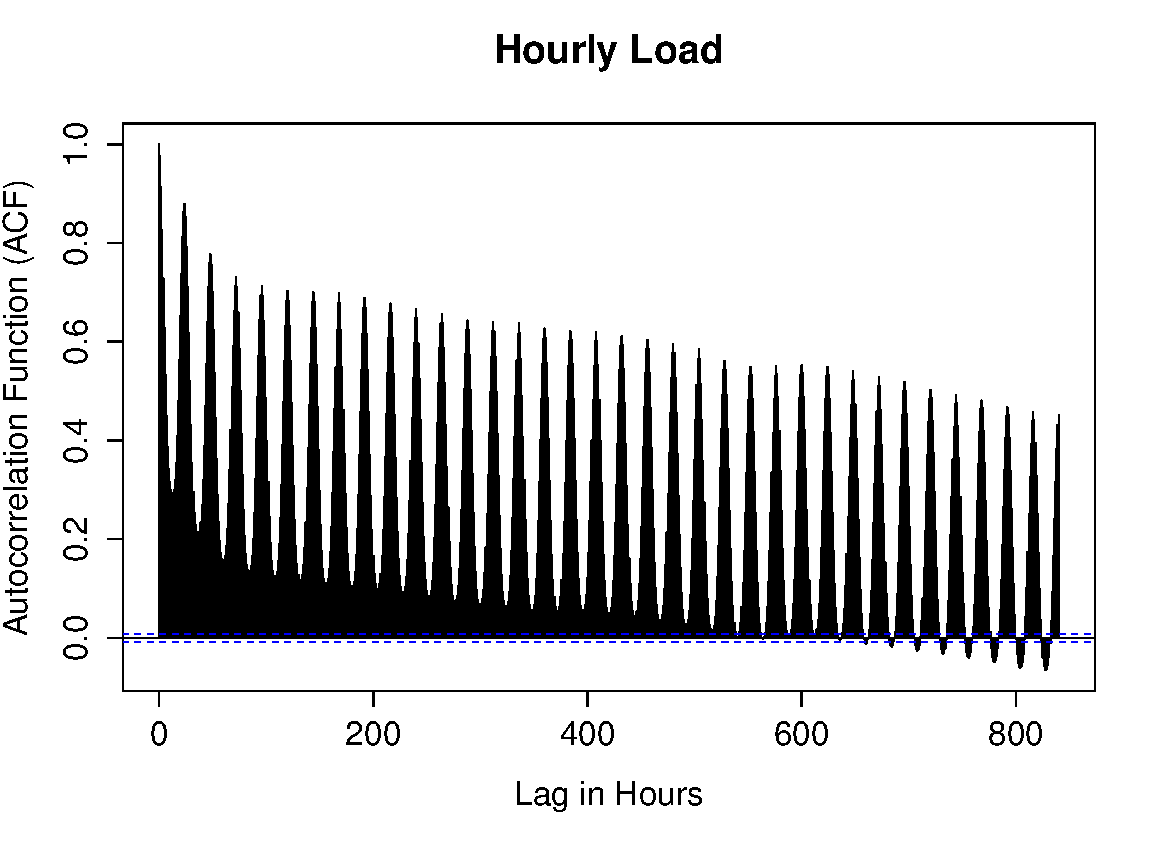
\includegraphics[width=\linewidth]{gfx/acf-load-35days.pdf}
\caption{35 days Autocorrelation}
\label{subfig:acf-load-7days}
\end{subfigure}
\caption{Autocorrelation Function Estimates for hourly load data in MW for different maximum lags}
\label{fig:acf-load}
\end{figure}

\subsection{Calendar Features}
\label{sec:calendar}
Figures \ref{fig:temp-lags} and \ref{fig:acf-load} have shown both temperature and load series to possess daily frequency. We therefore extract the hour of the day from the datetimes and use it as a feature. 

Figure \ref{fig:seasonality} demonstrates the seasonal change of temperature and load throughout the year. In order to capture the seasonality in our models for both temperature and load, we use the time of the year as a feature. We indicate the progress of the current year with a sequence $\text{TOY} \in [0,1]$ \cite{Fan2010}. We dropped the original categorical variable indicating the present month in favor of the time of year feature (validated by experiment.) 

\begin{figure}[!ht]
\centering
\begin{subfigure}[b]{.49\linewidth}
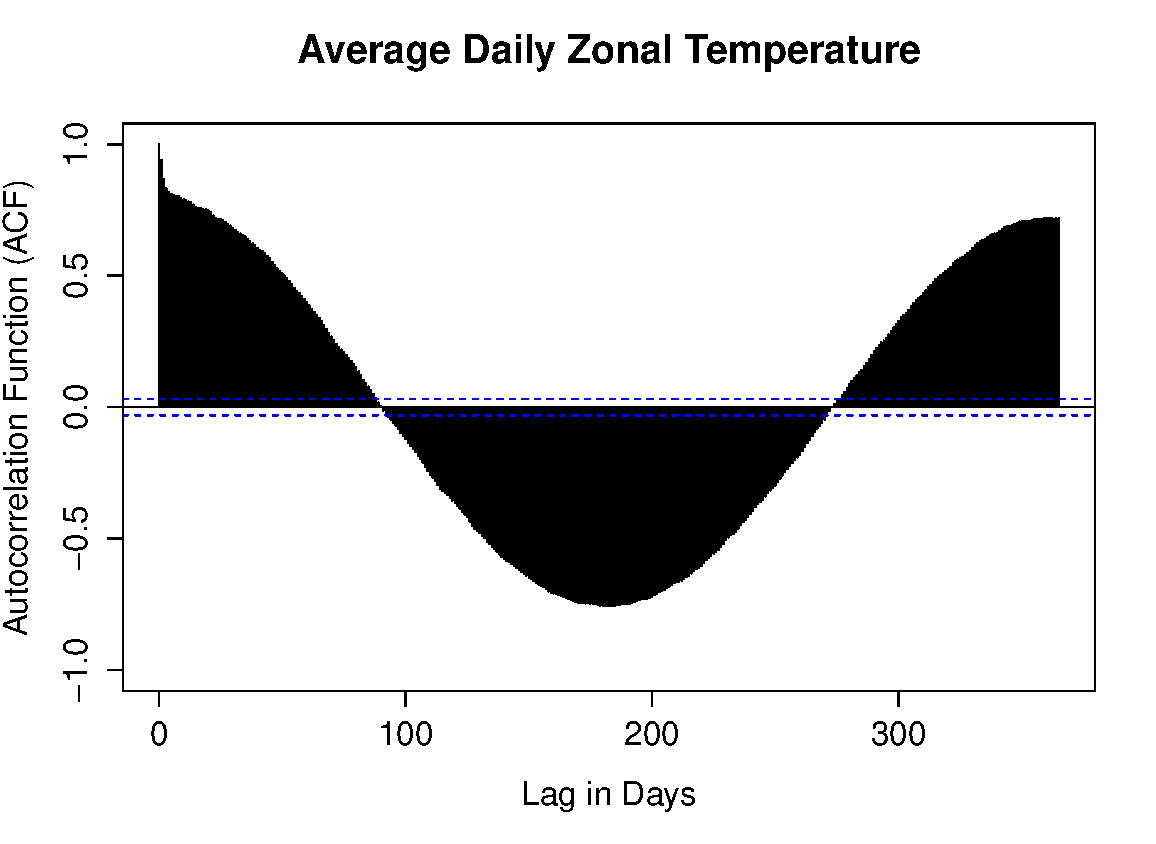
\includegraphics[width=\linewidth]{gfx/daily-avg-temp-1year.pdf}
\caption{Autocorrelation Estimates for daily average district temperature.}
\label{subfig:acf-temp-1year}
\end{subfigure}
\begin{subfigure}[b]{.49\linewidth}
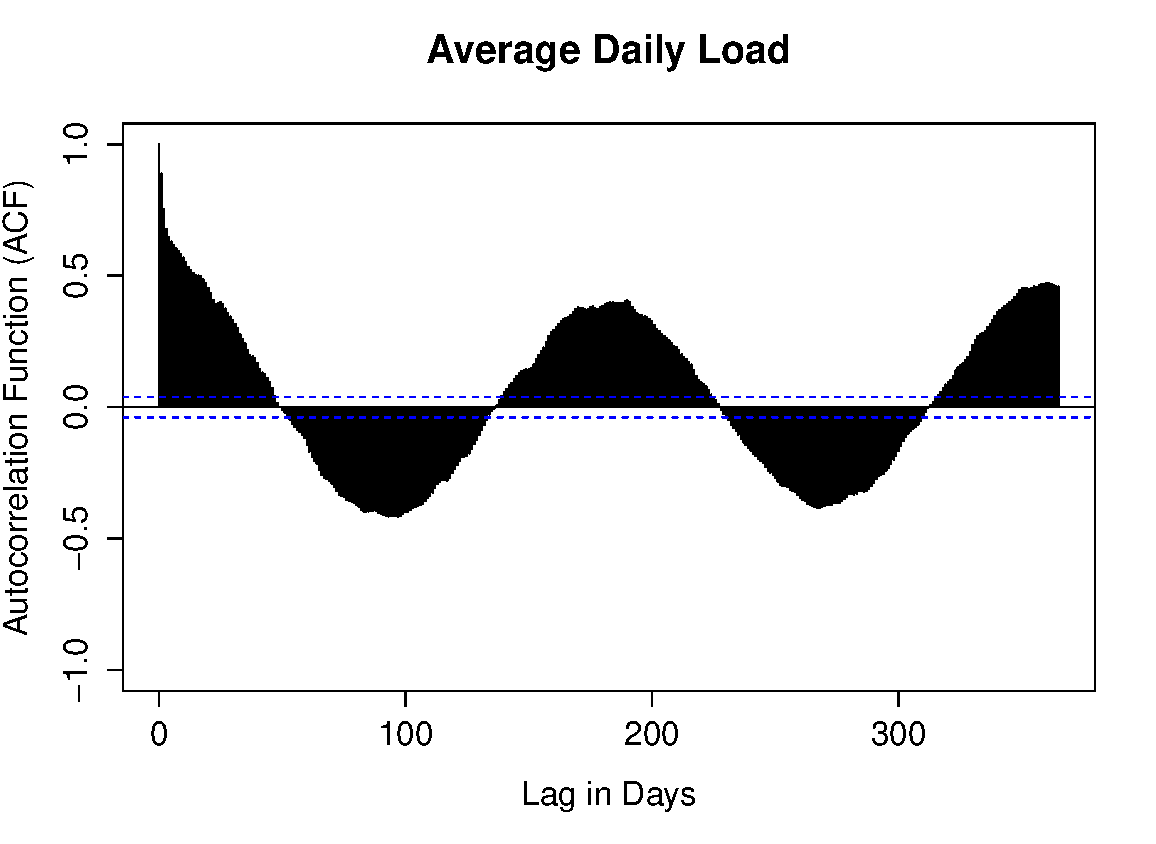
\includegraphics[width=\linewidth]{gfx/avg-daily-load-1year.pdf}
\caption{Autocorrelation Estimates for daily average district load.}
\label{subfig:acf-load-1year}
\end{subfigure}
\caption{Autocorrelation Function Estimates for daily averages of both district temperature and load for 1 year.}
\label{fig:seasonality}
\end{figure}
The features we discussed so far are proven useful for both temperature and load forecasting later in this report (Section \ref{}). The nature of the load data allows us to proceed with the extraction of another feature, the day of the week as introduced by \cite{Hong2010}. Energy consumption does not only depend on the climatic circumstances, but also directly on the calendar events, because consumption patterns vary between the different days of the week, weekends and holidays due to human activity (find source). The energy utility data does not show clear patterns when probing (Figure coming up). Nevertheless, as proposed in \cite{Hyndman2010} we use different approaches of marking the days of the week, numbering the days of the week from 1 (Sunday) to 7 (Saturday) and assigning weekdays and weekend days with 1 and 2 respectively.\par
The only external data source allowed for the GEFCom load forecasting track are \href{http://archive.opm.gov/Operating\_Status\_Schedules/fedhol/2014.asp}{U.S. federal holidays} for the time span of the provided data. This gives us the possibility to additionally detect holidays and assign them another integer (8) in the approach of consecutively numbering the days of the week.\par

\begin{table}[h]
\centering
\begin{tabular}{@{}lllllllll@{}}
\toprule
 & Mon & Tue & Wed & Thu & Fri & Sat & Sun & Holiday \\ \midrule
Weekdays vs -end & 2 & 2 & 2 & 2 & 2 & 1 & 1 & - \\
Weekdays & 2 & 3 & 4 & 5 & 6 & 7 & 1 & - \\
 & 2 & 3 & 4 & 5 & 6 & 7 & 1 & 8 \\ \bottomrule
\end{tabular}
\caption{My caption}
\label{my-label}
\end{table}

\section{Forecasting Methods}
(find paper using generative additive models for forecasting)
In this section we briefly review the forecasting models used during this project. On the one hand we use a generalization of the Linear Model (LM), the Generalized Additive Model (GAM), and on the other basic implementations of established machine learning methods such as Neural Networks (NN) and Random Forests(RF). Due to the limited scope of the project we did not use our own implementations, but rather those that have been made available through R packages.

instead of linear predictor refer to univariate response variable

\subsection{Linear Model (LM)}
We use the ordinary least squares (OLS) linear regression model as a benchmark method to interprete the prediction power of the other methods. OLS assumes the residuals to follow a normal distribution $\epsilon \sim \mathcal{N}(\mu, \sigma^2)$. The linear predictor is therefore the sum of a linear combination of covariates and Gaussian noise  and the predictor $y = \vec{\phi}^T \vec{x} + \epsilon$. The vector of covariates $\vec{x}$ contains the pre- selected features, i.e. the temperature variable and the calendar effects, as well as the bias term $x_0$ and $\vec{\phi}$ represents the vector of coefficients that are to be learnt with least squares approximation.

\subsection{Generalized Additive Model (GAM)}
Why do we use GAM?
The standard linear regression model we use is a generalized linear model with a gaussian distribution and an identity link function. For the general additive model \cite{Wood2006} we employ we will not change the link function, since we are going to use a Gaussian distribution here as well. However, generalized additive models allow a generalization on top of that of the incorporation of other distributions as in Generalized Linear Models, that of \emph{nonlinear predictors}. Hence, assuming a Gaussian error model the linear predictor turns into a nonlinear predictor with a combination of smooth functions of the predictor variables: $y=s_1(x_1)+s_2(x_2)+\dots+s_p(x_p)+\epsilon$, where the $s(x_i)$ are smooth functions of the chosen features. Note that not all covariates need to be wrapped in smooth functions.\par
Since the nonlinear functions are smooth they can be estimated by penalized regression in a spline basis \cite{Nedellec2014}, \cite{GAMS}:
\[
  s_i(x)=\sum_{j=1}^{k_i}\beta_{i,j}\varphi_j^i(x)
\]
Here $k_i$ is the dimension of the spline basis and $\varphi_j^q$ are the corresponding spline functions. The default splines for GAMs in the \textbf{mgcv} package are thin-plate splines \cite{Wood2003} where $\varphi(x)$ is of the family of radial basis functions. The focus of this project was on forecasting workflow and feature selection, so that different spline specifications have not been tried out.\par

Show model output and how degrees of freedom are chosen?

\subsection{Neural Network (NN)}
Neural networks are powerful machine learning algorithms. They exist in many varieties, with feedforward neural networks being the most basic. In our predictions we use a simple feedforward neural network with one hidden layer with a varying number of hidden units (from now on referred to as \textbf{hunits}) and a linear output unit. Such a network can be easily used for regression using the R package \emph{nnet} \cite{Venables2002}.

\subsection{Random Forest (RF)}
Random forests \cite{BreimanRF} are a powerful ensemble method for capturing nonlinear dependencies that does not require significant tuning. They employ decision trees which are very popular in machine learning. To avoid the effects of overfitting a bunch of random decision trees are automatically created and the mode of the probability density of the predictions is returned as the point predictions. We use the \emph{randomForest} R package \cite{Liaw2002} and try the algorithm for a varying number of trees. We will refer to this variable in the following as \textbf{ntrees}.

%case where the response is continuous and the covariates are both continuous and discrete.
%data \{yi,x1,i,...,xp,i; i = 1,...,n\}. In this short presentation, we focus on the
%The estimation is done by averaging many simple tree models. Each of the tree models is a recursive partitioning of the space of covariates, in order to obtain classes of observations that maximize some purity criterion for the response (e.g., reduce the intra-class variance). 
A decision tree can process continuous and discrete covariates, as is the case with our features, while providing a continuous response. Chapter 15 of \cite{hastie01statisticallearning} provides the reader with a detailed introduction to the subject. \textit{To do this, each simple tree gives its prediction, and these are then aggregated using the mean of the individual predictions. Each tree model assigns a class to the new vector of covariates, based on the recursive partitioning. Then, the prediction is the mean value of the responses that correspond to this class} \cite{Nedellec2014}.

%If the tree models are built to be de-correlated, the averaging step will reduce the variance of the random forest estimator significantly. In order to build a de-correlated tree model, the random forest adds two layers of controlled randomness to the data. The first layer is generated by a bootstrap sampling of the observations, while the second one is produced from a random draw from a subset of covariates on each partitioning step.
%For a new vector of covariates (x1,n+1 , . . . , xp,n+1 ), we can predict the value of the non-observed response yn+1 using the estimation fˆ of f , obtained using n data points. To do this, each simple tree gives its prediction, and these are then aggregated using the mean of the individual predictions. Each tree model assigns a class to the new vector of covariates, based on the recursive partitioning. Then, the prediction is the mean value of the responses that correspond to this class.

\section{Pipeline}

\subsection{Creation of Features}

\subsection{Crossvalidation}

\subsection{Monthly vs. Weekly}

\subsection{Creation of Quantiles}
We use the residuals $\xi=y-\hat{y}_i$ created during training to create the desired quantile forecast.
Error shoud ideally have zero mean
using model point predictions as the mean. 

\section{Analysis}
What combination of features and models for temperature and load provide us with a good prediction accuracy with respect to Gefcom leaderboard?

Structure analysis part to go
TODO:
\begin{itemize}
\item temperature CV bugS fixed
\item rerun temperature models
\item decide over effect of DLAG $\rightarrow$ effect on load models
\item choose temp method with best results, if similar results use one combination from every set
\item create additional droplets with 8 cores $\rightarrow$ install R, packages c("randomForest", "nnet", "mgcv"), git, htop $\rightarrow$ clone repository $\rightarrow$ rsync temperature data (DO NOT CREATE INSTANCE FEATURES DURING CV - checked)
\item run load LM with temperature PCA and Station1 of best model
\item test effect of different daytypes with GAM or LM?
\item if the two preceding cannot be tested before lunch, run all GAM, RF, NN models 
\item improve plotting, create residual plots, quantile plots etc. in loop
\item interprete results and create plots
\item write literature review (GAMs, Random Forest, NN (blackbox))
\item write conclusion
\end{itemize}


predtrain vs no pred train (GAM: LoadFormula 1, tempFormula 1)
$\rightarrow: weekly predtrain has better score, but only one position on average$

GAM: combined weekly temperature predictions worse than monthly prediction, model with DLAG slightly worse than without 

the first week is the worst on average
Combined weekly predictions better for GAM model! Does DLAG have positive effect? 

\subsection{Temperature Modeling}
\subsubsection{Data Processing}
average temperature vs. principal component

\subsubsection{Effect on Load Prediction}
Effect of temperature on load prediction evaluated using different methods:\\
Mean over past years (yearly lag), LM, GAM, NN, RF vs. true temperature

\subsubsection{Evaluate Results of weekly vs. monthly Temperature Prediction}
plot MAPE \& PINBALL scores for different methods over load training + CV period in a 1x2 plot of the form:\\
monthly scores \quad weekly scores

\subsection{Load Modeling}

\subsubsection{Evaluate the Influence of the Lag on Load Prediction}
set the basis by plotting MAPE \& PINBALL scores by week over w1, w2, w3, w4; one curve for every month in CV\\
do this for every method\\
as well as a comparison of the best performing configuration of every method among each other\\

\subsubsection{Evaluate Performance for different Method Configurations}
Use temp method that provides best score as shown in Temperature Modeling Section\par
Different GAM formulas:\\
plot MAPE \& PINBALL scores for all GAM formulas over CV period in a 2x2 plot of the form:\\
monthly load with monthly temp \quad monthly load with weekly temp\\
weekly load with monhtly temp \quad weekly load with weekly temp\par
\vspace*{5pt}
Different NN hidden units:\\
plot MAPE \& PINBALL scores in 2x2 plot\par
Different RF ntrees:\\ 
plot MAPE \& PINBALL scores in 2x2 plot\par

\subsubsection{Compare Performance of different Methods}
choose best scoring configuration for every method and plot the results in one 2x2 plot

% An example of a double column floating figure using two subfigures.
% (The subfig.sty package must be loaded for this to work.)
% The subfigure \label commands are set within each subfloat command, the
% \label for the overall figure must come after \caption.
% \hfil must be used as a separator to get equal spacing.
% The subfigure.sty package works much the same way, except \subfigure is
% used instead of \subfloat.
%
%\begin{figure*}[!t]
%\centerline{\subfloat[Case I]\includegraphics[width=2.5in]{subfigcase1}%
%\label{fig_first_case}}
%\hfil
%\subfloat[Case II]{\includegraphics[width=2.5in]{subfigcase2}%
%\label{fig_second_case}}}
%\caption{Simulation results}
%\label{fig_sim}
%\end{figure*}

\section{Conclusion}
The conclusion goes here.

\bibliographystyle{IEEEtran}
\bibliography{references}{}

\end{document}


